\documentclass[
	a4paper, % Paper size, use either a4paper or letterpaper
	10pt, % Default font size, can also use 11pt or 12pt, although this is not recommended
	unnumberedsections, % Comment to enable section numbering
	twoside, % Two side traditional mode where headers and footers change between odd and even pages, comment this option to make them fixed
]{LTJournalArticle}
\usepackage{amsmath}
\usepackage{multirow}
\addbibresource{refs.bib} % BibLaTeX bibliography file

% A shortened article title to appear in the running head, leave this command empty for no running head

% \footertext{\textit{Journal of Biological Sampling} (2024) 12:533-684} % Text to appear in the footer, leave this command empty for no footer text

\setcounter{page}{1} % The page number of the first page, set this to a higher number if the article is to be part of an issue or larger work

%----------------------------------------------------------------------------------------
%	TITLE SECTION
%----------------------------------------------------------------------------------------

\title{Probabilistic Approaches to 
\\ Energy Conservation in CDNs} % Article title, use manual lines breaks (\\) to beautify the layout

% Authors are listed in a comma-separated list with superscript numbers indicating affiliations
% \thanks{} is used for any text that should be placed in a footnote on the first page, such as the corresponding author's email, journal acceptance dates, a copyright/license notice, keywords, etc
\author{%
	Adarsh Hiremath, Artemas Radik, Andrew Palacci \\
	CS 262: Introduction to Distributed Systems \\
}


%----------------------------------------------------------------------------------------
\newtheorem*{remark}{Remark}
\begin{document}

\maketitle % Output the title section

%----------------------------------------------------------------------------------------
%	ARTICLE CONTENTS
%----------------------------------------------------------------------------------------

\section{1. Introduction}
Over the past semester, we've learned about the fundamentals of distributed systems, their implementations, and their uses. We were particularly interested in the idea of replication as it relates to  For this paper, we sought to find an application of the replication that we learned that went beyond fault-tolerance, and provided additional benefits to the companies or individuals implementing them. with this project, these benefits are twofold — we show that companies implementing CDNs for content delivery are not only able to deliver content faster (the primary goal) but also more energy-efficiently. in a time where the climate is clearly becoming more at risk and legislation is also beginning to respond, we decided that CDNs were a great place to make advances as to their energy efficiency”

Before we make any 

In this paper, we explore several gaps in the literature as to energy efficiency in CDNs, and make three key contributions:
\begin{enumerate}
    \item We more rigorously examine the choice of various probability distributions and parameters as cache policies for CDNs, by relating them to the various content categories available online today.
    \item We redefine an existing model and constraints to be more flexible and closely aligned with the needs and consumption of modern CDNs.
    \item We provide a strategy and code for modeling an appropriate amount of surrogate servers that should be used for a CDN with given characteristics --- namely, we do this by finding a \textit{crossover point} where a CDN's overall energy consumption begins to increase.
\end{enumerate}
% brief explanation of what CDNs are and what they are typically used for
% the novel contributions of this paper are: A. fitting to different distributions B. new probability calculations C. a way to calculate

\section{2. Existing Approaches}

Several recent papers cover the topic of energy consumption in CDNs. Paper \cite{ulIslam2012} proposes a new energy consumption model for CDN surrogates, compares Uniform and Zipfian client redirection policies, and simulates results via a CDNSim testbed \cite{cdnsim}. Critically, the model introduced in \cite{ulIslam2012} does not incorporate network synchronization or transmission costs into it's energy model, opting to instead dismiss them. 

Paper \cite{osmanthesis} does account for costs such as that of transmission energy, but also has a general focus on determining optimal CDN cache sizes (both fixed and variable) via a proposed mixed-integer linear programming model. Notably, \cite{osmanthesis} does not have an apparent focus on optimizing CDN surrogate quantities at scale.

Unlike \cite{osmanthesis} and \cite{ulIslam2012}, paper \cite{biancoCDNs2017} assumes that CDN cache sizes are a constant factor of the primary in order to analyze transmission, synchronization, and other costs in-depth. We were able to closely replicate the findings of \cite{biancoCDNs2017}, with small quantitative differences but identical qualitative conclusions. Their model — which is the basis for our proposed model — aligns closely with the reality of the internet. As a result, it's key to understand their approach, which is outlined in the remainder of this section.

\subsection{2.1. Network Topology}

We represent a CDN as a \textit{primary} server, storing the entire data set, connected to several \textit{surrogate} servers, each of which store a fixed-size randomized subset of the primary's contents. The idea is that surrogates sit on the network edge, closer to end users — minimizing cost, latency, and energy usage. 

Both the primary and surrogates sit in the internet, which at large can be modeled as a three-tier network of ISPs (Internet Service Providers). Each tier can be described as follows:
\begin{enumerate}
    \item Tier one ISPs have global reach and are at the top of the hierarchy.
    \item Tier two ISPs are typically regional or country-based, and are responsible for connecting between tier one and tier three ISPs.
    \item Tier three ISPs provide internet connectivity to end users.
\end{enumerate}

\begin{figure}[h]
	\begin{center}
		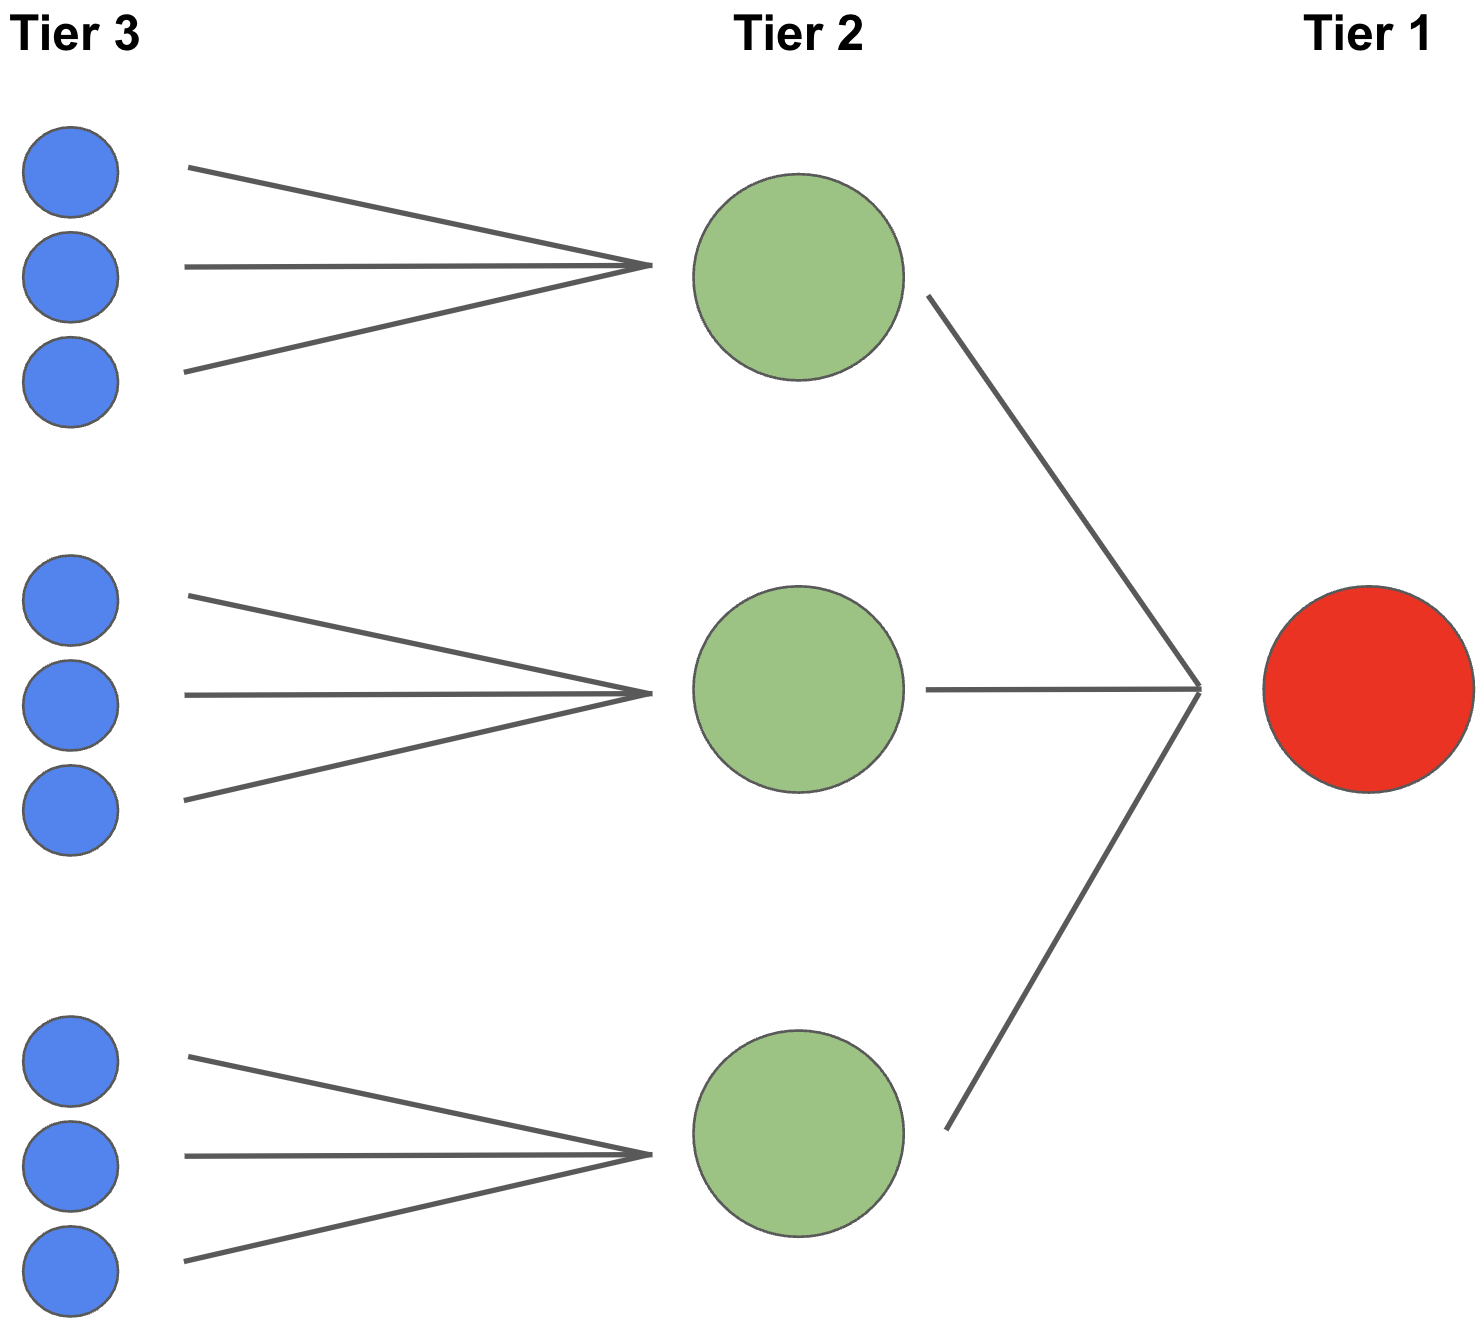
\includegraphics[width=8.1cm]{tier-2.png}
	\end{center}
	\caption{A simplified three-tier ISP topology.}	
\end{figure}

In our model, there are $S$ surrogate servers randomly distributed according to a uniform distribution across all tier three ISPs, with $S < T_2$, the number of tier two ISPs. It is assumed that each tier two ISP is limited to at most one surrogate server in one of its connected tier three ISPs. The graphic below illustrates a tier one ISP as the green bubble, tier two ISPs as orange bubbles, and tier three ISPs as red bubbles. Black squares are surrogate servers, and the primary server is available only via tier one.

\begin{figure}[h]
	\begin{center}
		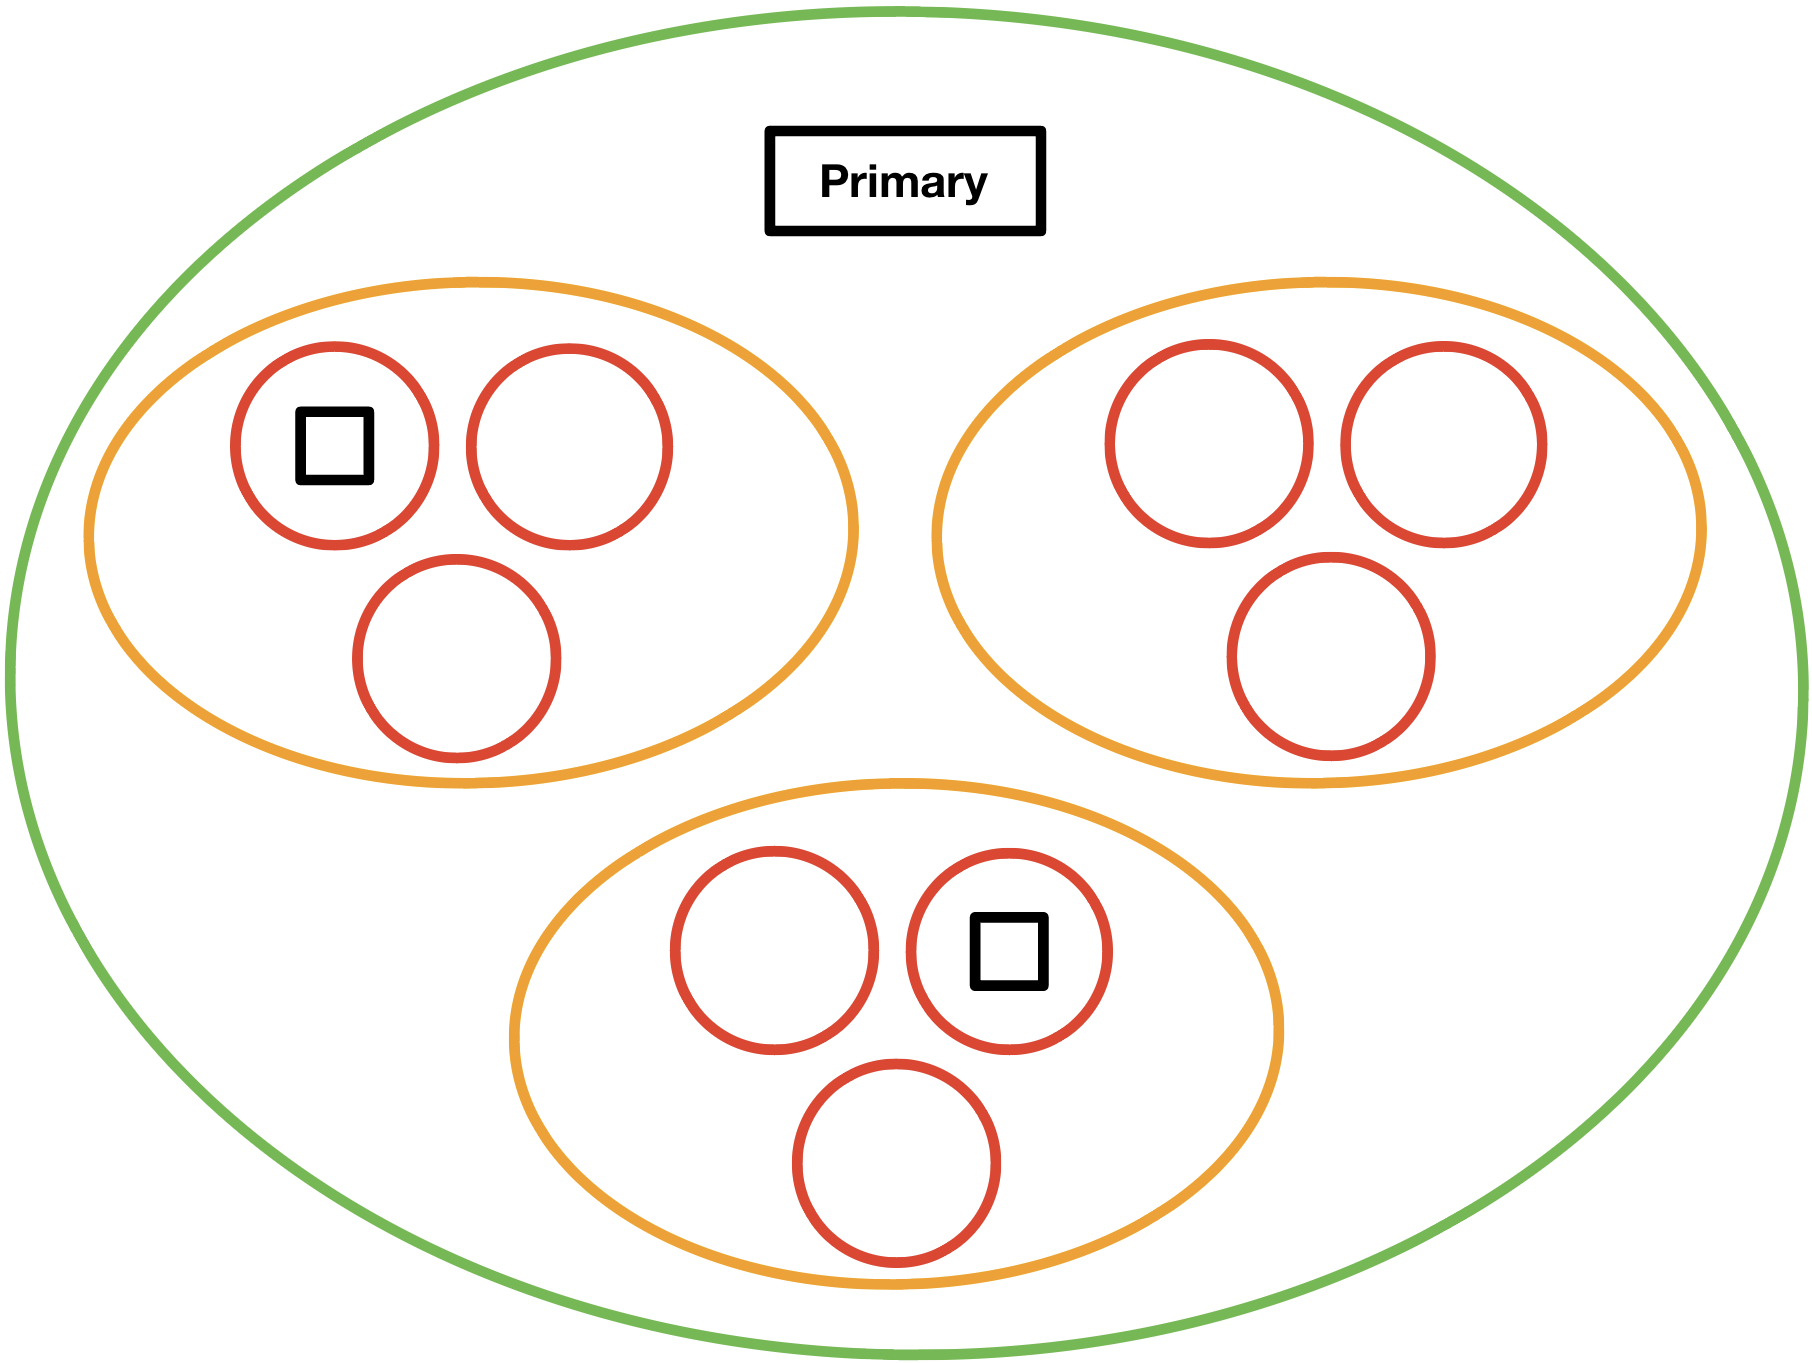
\includegraphics[width=8.1cm]{bubble.jpeg}
	\end{center}
	\caption{Surrogate server constraints visualized in the three-tier ISP topology.}	
\end{figure}
\begin{remark}
The $S < T_2$ constraint is used in the existing literature, though it is rather unintuitive and indeed a limitation of the existing models. Our proposed modifications and calculations, introduced later on, remove the need for this constraint.
\end{remark}



% Efficiently caching content is crucial for highly performant CDNs. Web multimedia data such as text, video, and audio can be exceptionally large, making cache policies essential for ensuring that clients receive data quickly without overburdening the surrogate servers in the CDN. In a simple 3-tier CDN model, we want to move the most popular content to the surrogate servers in the furthest edge of the network - in this case, the 3rd tier.  

% \begin{figure}[h]
% 	\begin{center}
% 		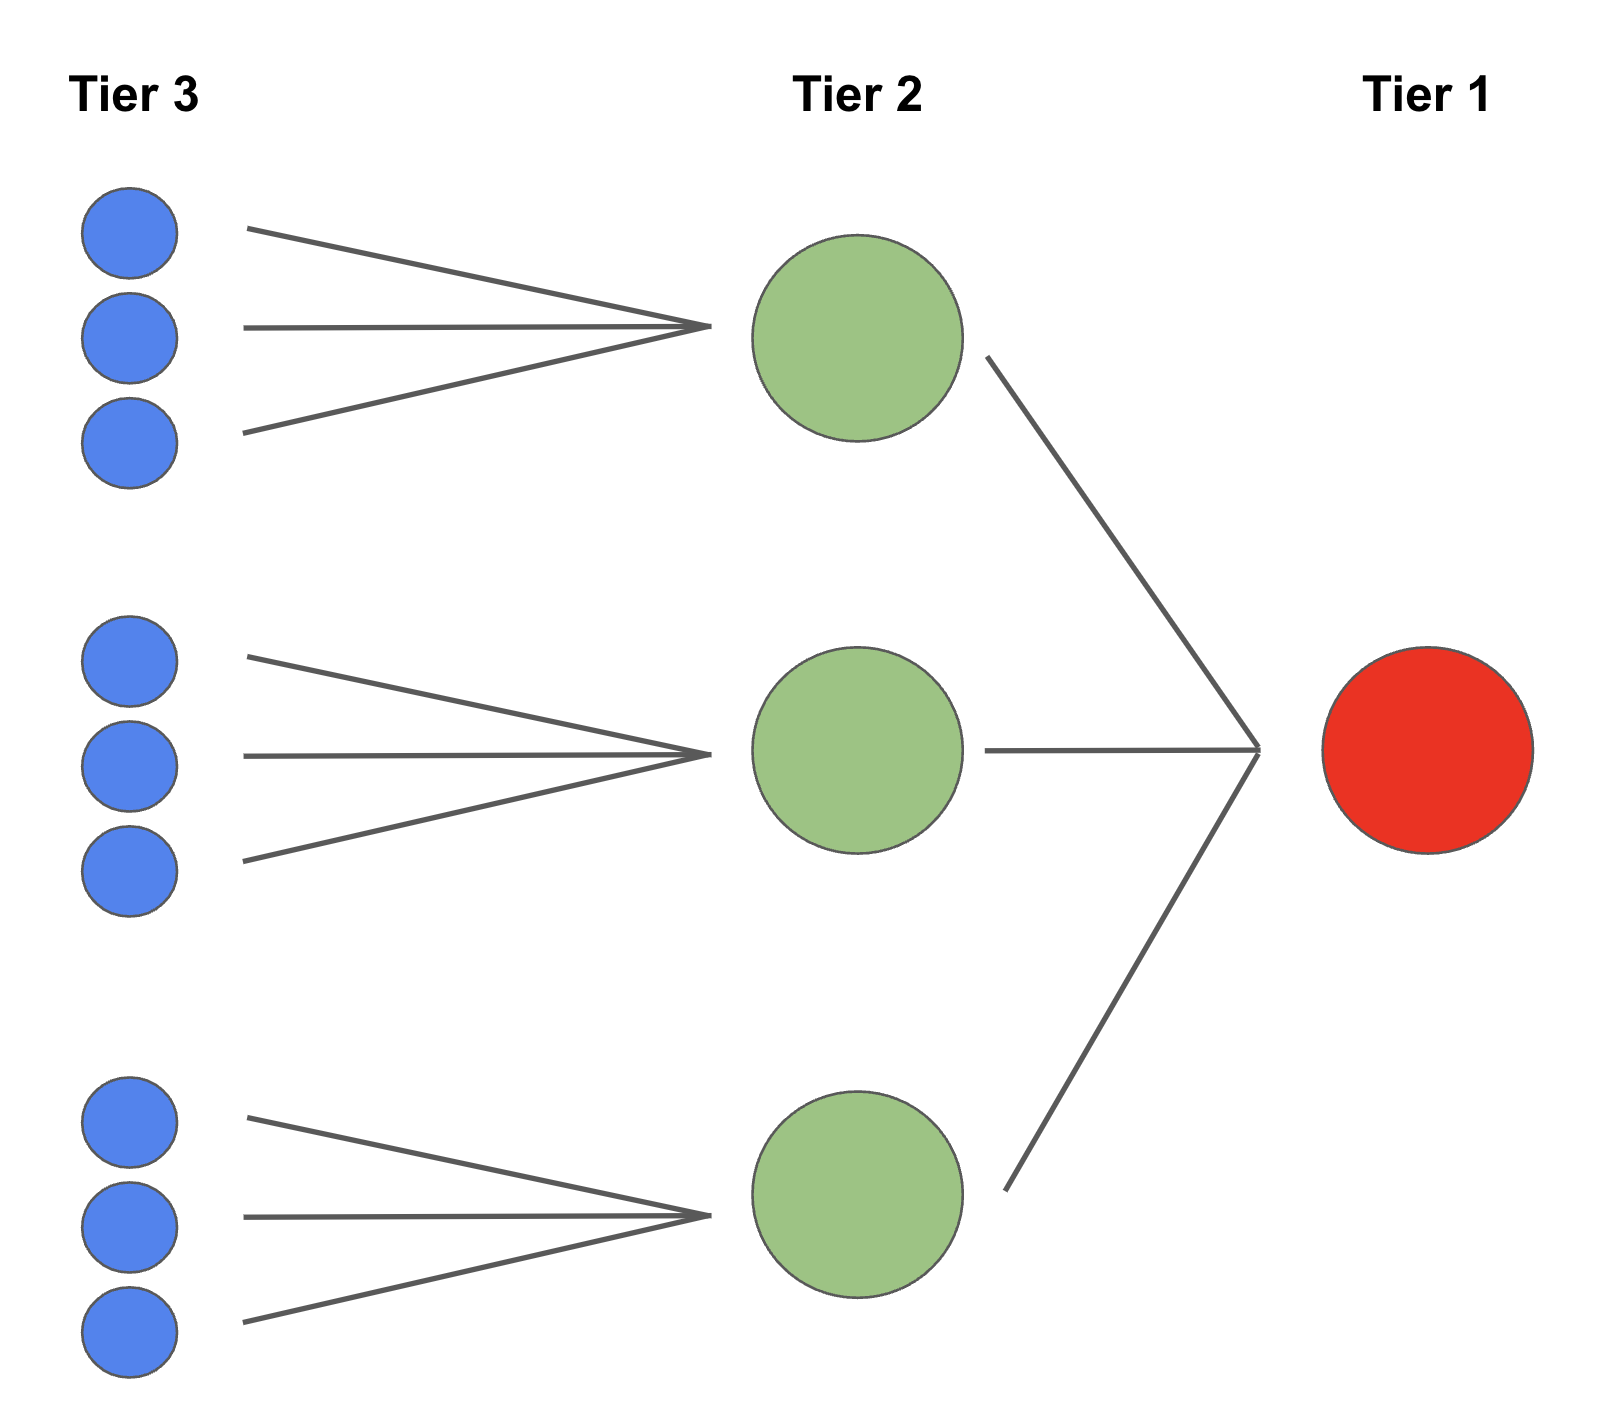
\includegraphics[width=8.1cm]{tier.png}
% 	\end{center}
% 	\caption{A caption for this image.}	
% \end{figure}

% Throughout the paper, we reference the above $3$-tier model. We note the following assumptions and notations about the model: 
% \begin{itemize}
% 	\item Each node in the above model is an ISP. The surrogate servers are placed \textit{within} a tier 3 ISP.
% 	\item The primary server contains all of the content in the CDN, and propagates modified/new content to surrogates according to the cache policy. 
% 	\item There are $T_1$ ISPs in tier $1$, $T_2$ ISPs in tier $2$, and $T_3$ ISPs in tier $3$. 
% 	\item There are $S$ surrogate servers. 
% 	\item $g_3$ represents a group of Tier $3$ ISPs. 
% 	\item The hit probability for each surrogate server is represented as $P_{hit}$.  
	
% \end{itemize}

\subsection{2.2. Cache Policies}
Our model utilizes a cooperative push-based approach, where content is pushed by the primary to each of the surrogates beforehand. The primary keeps a mapping between content and servers, and directs requests accordingly. 

The key problem that cache policies address is how the primary server should allocate content across the available surrogates. Ideally, content is distributed in such a way that maximizes cache hit ratios and (thus) minimizes energy costs.

The first approach requires selecting the data to be stored in each surrogate according to a uniform distribution among the entire data set. In other words, the primary server chooses a random subset of its content to allocate to each surrogate. 

The second approach is popularity-based, and requires as a prerequisite that the primary has an exact ranking of each content's popularity values (these can be view counts, like counts, etc). The data to be stored in each surrogate is randomly selected according to a Zipf distribution with parameter $\alpha = 0.8$. This works because it is shown that many web platforms have content access patterns following an identical distribution \cite{749260}.

\begin{figure}[h]
	\begin{center}
		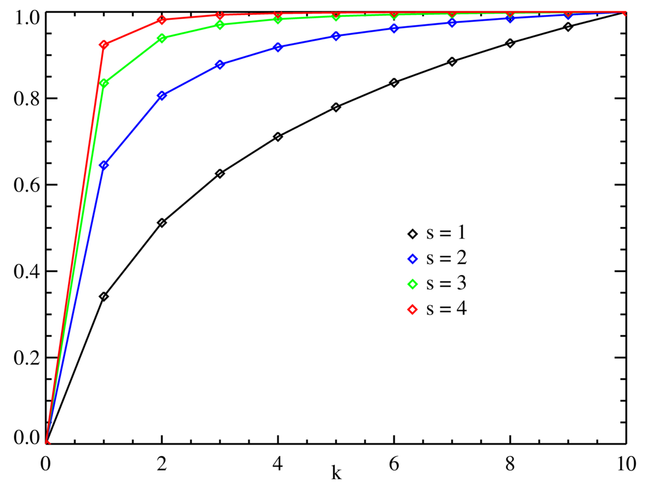
\includegraphics[width=8.1cm]{zipf.png}
	\end{center}
	\caption{A graph of the Zipf distribution CDF with support $k\in\{1, 2, \ldots, 10 \}$ for multiple parameters $s=\alpha \in \{1,2,3,4\}$}.
\end{figure}

\begin{remark}
    Zipf with parameter $\alpha=0.8$ is not always accurate, as later sections will show. This is yet another limitation of the models proposed in existing literature.
\end{remark}

\subsection{2.3  Hit Probability}

The hit probability is the probability that a surrogate server incurs a cache hit. For the uniform approach, the hit probability is trivial: it is simply the size of the surrogate cache as a fraction of the primary storage size. By \cite{749260} and basic probability, the hit probability for the Zipf approach is as follows:

\[ P_{hit}(\alpha, c, n) = \sum_{i=1}^{cn} \frac{\left( \sum_{k=1}^{n} \frac{1}{k^\alpha}\right)^{-1}}{i^\alpha} = \frac{H_{}}{} \]

\subsection{2.4  Modeling Energy Consumption}
\begin{center}
\begin{table}[h]
\scriptsize
\begin{tabular}{ |c|c|c| } 
 \hline
 Symbol & Default Value & Description \\ 
 \hline
 $S$ & variable & number of surrogate servers \\ 
 \hline
 $S_C$ & 40\% & surrogate cache size (relative to primary) \\ 
 \hline
 $M$ & 1000 & total number of contents stored \\ 
 \hline
 $B$ & $10^6$ bits & size of one content \\ 
 \hline
 $t$ & 6000 s & duration of our analysis \\ 
 \hline
 $n_m$ & $S_c \cdot S$ & number of replicas of content $m$ \\ 
 \hline
 $r_m$ & 100, 1000, 10000 & average requests for content $m$ \\ 
 \hline
 $m_m$ & 10, 100 & average modifications for content $m$ \\ 
 \hline
 $H^A_{sd}$ & 3 & hops to fetch content in same Tier 3 ISP \\ 
 \hline
 $H^B_{sd}$ & 14 & hops to fetch content in same Tier 2 ISP \\ 
 \hline
 $H^C_{sd}$ & 25 & hops to fetch content from core network \\ 
 \hline
 $H_{ps}$ & $H^C_{sd}$ & hops from primary to a surrogate \\ 
 \hline
 $T_3$ & 1000 & number of Tier 3 ISPs \\ 
 \hline
 $g_3$ & 20 & number of Tier 3 ISPs per Tier 2 ISP \\ 
 \hline
 $T_2$ & 50 & number of Tier 2 ISPs \\ 
 \hline
 $P_{st}$ & $7.84 \cdot 10^{-12}$ W & storage energy usage per bit \\ 
 \hline
 $E_r$ & $1.2 \cdot 10^{-8}$ J/bit & router energy usage per bit \\ 
 \hline
 $E_l$ & $1.48 \cdot 10^{-9}$ J/bit & link energy usage per bit \\ 
 \hline
 $E_{sr}$ & $2.81 \cdot 10^{-7}$ J/bit & server energy usage per bit \\ 
 \hline
\end{tabular}
\caption{Parameter values for the existing version of our model.}
\end{table}
\end{center}
\normalsize
\[E_{tot} = E_{storage} + E_{server} + E_{synch} + E_{tx}\]
\[E_{storage} = \sum_mBn_mP_{st}t\]
\[E_{server} = \sum_mBr_mP_{sr}\]
\[E_{synch} = \sum_mBm_mn_m[E_r(H_{ps} + 1) + E_l(H_{ps})]\]
\[P_A = \frac{S}{T_2} \cdot \frac{1}{g_3} \cdot P_{hit}\]
\[P_B = \frac{S}{T_2} \cdot \left(1 - \frac{1}{g_3}\right) \cdot P_{hit}\]
\[P_C = 1 - (P_A + P_B)\]
\begin{multline*}
    E_{tx} = P_A\sum_mBr_m[E_r(H^A_{sd} + 1) + E_l(H^A_{sd})] \\
      + P_B\sum_mBr_m[E_r(H^B_{sd} + 1) + E_l(H^B_{sd})] \\
      + P_C\sum_mBr_m[E_r(H^C_{sd} + 1) + E_l(H^C_{sd})] \\
\end{multline*}

\subsection{2.5  Results}
\begin{figure}[h]
	\begin{center}
		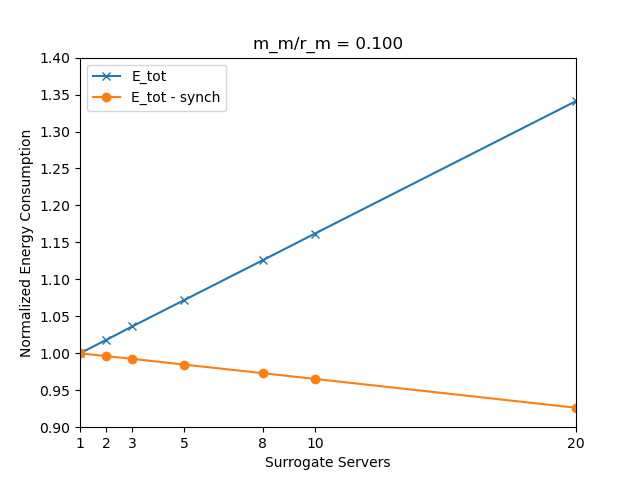
\includegraphics[width=8.1cm]{plots/sc40ratio0.1zipf.png}
            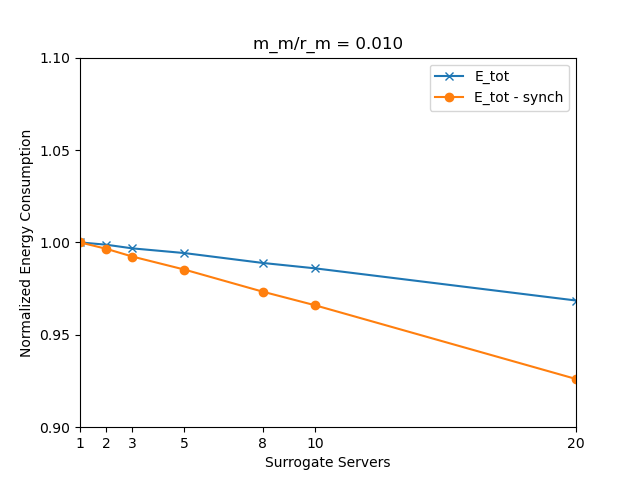
\includegraphics[width=8.1cm]{plots/sc40ratio0.01zipf.png}
	\end{center}
	\caption{Graphs of $E_{tot}$ and $E_{tot - synch}$ for a Zipf cache policy, with a modify/request ratio of $0.1$ (top) and $0.01$ (bottom), and a cache rate of $40\%$.}	
\end{figure}


\section{3. A Better Cache Policy}

While \cite{biancoCDNs2017} asserts that Zipf with $\alpha = 0.8$ is an accurate caching policy for a variety of multimedia, content distributions on modern platforms like Tik Tok, Spotify, and YouTube all have different viewership patterns. This suggests that in some cases Zipf with $\alpha = 0.8$ may not be the best caching policy and alternate distributions could offer a better framework for CDN caching. 

Since platforms like Tik Tok and Spotify contain more items with high popularity and more items that spontaneously change in popularity by going viral alright, the distribution of popularity may be less skewed than Zipf with $\alpha = 0.8$ might suggest. Therefore, using the Zipf distribution to determine cache allocation especially for short-form video content may not be as effective as for other types of multimedia. Additionally, since short-form video content requires larger amounts of storage space, efficient cache allocation modeling is even more crucial to ensure optimal performance of a CDN. 

Instead of using Zipf with $\alpha = 0.8$, we build off of \cite{osmanthesis} and propose dynamically adjusting $\alpha$ based on different multimedia patterns. 

\subsection{3.1 Shortfalls of Zipf}

Popular platforms like Spotify and Tik Tok have an extremely high viewership rates. Spotify, for example, has $489$ million monthly active users. Since the average Spotify user listens to approximately $720$ songs per month, we can estimate total monthly traffic as follows: 
\[
	489,000,000 \cdot 720 = 352.08 \texttt{ billion listens}
\]  
	
The most streamed Spotify song ever currently has $3.335$ billion streams. Averaged on a per-month basis since its release date in $2019$, we get $79,404,761$ monthly streams. Thus, on a given month, this song would be streamed with probability: 
\[
	\frac{79,404,761}{352,080,000,000} \approx 0.0023.
\] 

However, the Zipf distribution suggested by \cite{biancoCDNs2017} underestimates this probability. Recall that the frequency of viewership with a Zipf distribution for $i$ content objects ranked $i = 1, 2, \ldots, N$ is

\[
	P_N(i) = \frac{\Omega}{i^{\alpha}}
\] 

where 

\[
	\Omega = \left(\sum_{1}^{N} \frac{1}{i^{\alpha}}\right)^{-1}
\] 

by \cite{749260}. Since \cite{biancoCDNs2017} asserts that we should use parameter $\alpha = 0.8$, we fix $\alpha = 0.8$ for all our calculations with Zipf. 

Since there are approximately $80$ million songs on Spotify, Zipf would indicate that the probability of a stream on a given month being the most streamed song should be 

\[
	P_{80,000,000}(1) = \frac{\left(\sum_{1}^{80,000,000} \frac{1}{1^{0.8}}
	\right)^{-1}}{1^{0.8}} \approx 0.0000000125 \
\] 

which is an underestimate by a very large margin compared to our original calculation of $0.0023$.

Clearly, in the case of Spotify, the assertion that using Zipf with $\alpha = 0.8$ accurately captures content popularity patterns does not hold. These probability errors continue to compound for $i = 2, 3, 4, 5, \ldots, N$ because distances between the most popular types of content aren't consistent with what Zipf with $\alpha = 0.8$ would indicate. 

As \cite{osmanthesis} suggests, different popularity distributions of cached content exist in different video services. In order to optimize power and delay of video delivery, the ideal content to store in caches should be determined using the popularity distribution instead of relying solely on arbitrarily-distributed popularities according to Zipf ($\alpha$ = 0.8) as suggested by \cite{biancoCDNs2017}. 

For example, Real TV viewing data indicates that when the diversity of video popularities is high, storing the few most popular videos in caches minimizes power consumption, with power savings of up to 72\%. However, when video popularities are similar, the best power efficiency is achieved by maintaining variable caches in the network. In the context of the Zipf distribution, similarly popular video similarities might mean increasing the value of $\alpha$ to ensure the first ranked item isn't assigned an extremely high probability of a hit.


\subsection{3.2 Calculating Hit Probability}



\subsection{3.3 Pareto Parameter vs. Hit Probability}

In this section, we attempt to use a Pareto distribution with varying alpha values to demonstrate the impact on $P_{hit}$ calculations. For example, with an $\alpha = 1.16$ parameter, the Pareto principle (also known as the $80/20$ rule) would dictate that that 20\% of the content is responsible for 80\% of the views. This might be appropriate for certain types of content, such as movie streaming after a set of popular movie releases, which is why holding $/alpha = 0.8$ does not make sense. 

The Pareto distribution is essentially a continuous version of the Zipf distribution. The probability mass function (PMF) of the Pareto distribution can be mathematically expressed as:

\[
    P(X \geq x) = \left(\frac{x_m}{x}\right)^\alpha
\]

where $X$ is a random variable representing the size of a file, $x$ is the threshold size for caching, $x_m$ is the minimum file size for caching, and $\alpha$ is a parameter that controls the skewness of the distribution. Like the Zipf distribution, the Pareto distribution is a power law distribution, meaning that the ratio of frequencies of any two elements in the distribution is independent of the elements' actual values.  

\begin{figure}[h]
	\begin{center}
		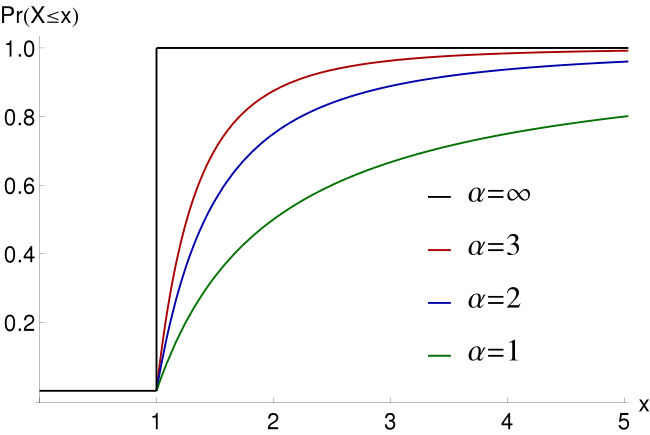
\includegraphics[width=8.1cm]{pareto.png}
	\end{center}
	\caption{A graph of the Pareto distribution CDF for various $\alpha$ with a scale parameter of $1$.}	
\end{figure}

The graph of the cumulative distribution function (CDF) of the Pareto distribution very strongly mirrors the Zipf distribution because both distributions are monotonically decreasing and positively skewed. 

\subsection{3.4 Pareto-based Energy Consumption (RESULTS)}

\section{4. Adaptations to Larger CDNs}
So far, the CDN energy consumption model we reference has been very useful for observing how to seek greener content delivery, alongside how using various cache policies affects energy usage. However, while working with the model, we also found some of our original assumptions and constraints to be unintuitive. In this section, we first examine the constraint on the amount of surrogates in our model, and then examine an important missing factor in our energy consumption calculations.

\subsection{4.1 Relaxing Surrogate Constraints}
Our above model makes the assumption that $S < T_2$ --- that there are fewer CDN surrogate servers than Tier 2 ISPs, and furthermore that there exists at most one surrogate per Tier 2 ISP. Reminding ourselves that in a realistic Internet hierarchy, Tier 2 ISPs are regional and national providers that operate both closer to clients than Tier 1 ISPs but further than Tier 3 ISPs, this assumption is unrealistic. If a large provider (e.g. TikTok or Spotify) wanted to rapidly deliver content, it would obviously want to have surrogates at as many Tier 3 ISPs as possible, regardless of whether they are connected to the same Tier 2 ISP. 

Furthermore, recalling our goal of optimizing CDN energy consumption, the results we found in previous sections seem to illustrate that adding surrogate servers consistently contributes to decreased normalized energy consumption. We realized this clearly couldn't be true, both in our model and in reality --- once there exists a surrogate in each Tier 3 ISP, there is no way to lower the amount of hops from a client to a surrogate. The only potential benefit of having several surrogates in a single Tier 3 ISP is redundancy, which we do not seek here because surrogates only contain part of the existing content, and our primary server is assumed to be stable. 

Given these two findings, we sought a way to update our constraint such that $S \leq T_3$ instead --- this follows from the fact that it could potentially be useful, and even energy-efficient, to continue adding surrogates until there is a surrogate at each Tier 3 ISP. As a result, we restructured our transmission energy consumption in order to allow for this new constraint. Namely, the probabilities $P_A, P_B, P_C$ of a client's closest hit being at a Tier 3, 2, or 1 ISP must be changed accordingly. 

For the purpose of interpretability, we shall assume that new surrogates will be uniformly randomly assigned to a Tier 3 ISP. Of course, this is not an entirely accurate assumption to make, since some Tier 3 ISPs have far higher priority than others, such as ones in more in-demand geographic areas (New York instead of Montana) or ones with a greater service population. However, our model already makes similar implicit assumptions, such as the fact that clients and surrogates are evenly geographically distributed. Furthermore, our model focuses on differentiating costs \textit{between} ISP tiers, and not \textit{within} them, so we shall leave this part to Future Work.

First, we calculate $P_A$ --- the probability that when a client requests a given piece of content, there exists a surrogate in the same Tier 3 ISP and it has that content. Here, we simply multiply the probability of a surrogate existing in that Tier 3 ISP ($\frac{S}{T_3}$ by uniformity) and the probability of a cache hit ($P_{hit}$, as calculated earlier). This gives us:
\[P_A = \frac{S}{T_3} \cdot P_{hit}\]
Next, we calculate $P_B$ --- the probability that the content could not be retrieved from a surrogate in the same Tier 3 ISP, but was able to be retrieved from a surrogate in the same Tier 2 ISP. First, we define a random variable for the amount of surrogates in a given Tier 2 ISP --- based on uniform selection without replacement, this gives us:
\[S_2 \sim \textrm{HGeom}(S, T_3-s, g_3)\]
Then, in order to formulate $P_B$, we summate over the amount of surrogates in a Tier 2 ISP where it is possible that a hit occurs --- this is 1 to $g_3$, since there cannot be a hit with 0 surrogates and there can also be at most 1 surrogate per Tier 3 ISP. Next, at each value in the summation, we calculate the probability of a hit for a Tier 2 ISP with that many surrogates --- this is $(1 - (1 - P_{hit})^i)$, since $(1 - P_{hit})^i$ defines the probability of none of the $i$ surrogates containing the requested content. Finally, we note that this summation includes scenario $A$, so we incorporate this to address overcounting:
\[P_B = \sum^{g_3}_{i=1}[P(S_2 = i) \cdot (1 - (1 - P_{hit})^i)] - P_A\]
\[P_B = \sum^{g_3}_{i=1}\left[\frac{\binom{S}{i}\binom{T_3-S}{g_3 - i}}{\binom{T_3}{g_3}} \cdot (1 - (1 - P_{hit})^i)\right] - P_A\]
Finally, $P_C$ accounts for the scenario that neither of the above occurred, and thus it is calculated as follows:
\[ P_C = 1 - (P_A + P_B)\]
Although this has ramifications on $E_{tx}$ as described above, our model otherwise remains unchanged. However, this opens up a new range of possible values for $S$, which is now constrained by $0 \leq S \leq T_3$ --- in 4.3, we shall see that this expanded range proves insightful.

\subsection{4.2 Incorporating Idle Energy Costs}
Another assumption made was that servers only incurred an energy cost whenever actively processing a client's request. Although for larger CDNs this may effectively be true (since they are constantly performing computations),  we believe it is important to include an idle energy, even if it is minimal relative to the other forms of energy consumption in a CDN. This incorporates an element of \cite{ulIslam2012}, which emphasizes the use of idle power as a potentially crucial aspect of CDN server utilization and energy consumption.

As a result, we shall also slight
\subsection{4.3 Results}
After incorporating the new modeling of $E_{tx}$ using $P_A, P_B, P_C$, and accounting for idle energy as described in 4.2, we can observe some new trends in our data that differ from what we find in 2.5. 


\section{5. Conclusions}

Before developing our own adaptations and models for energy usage in CDNs, we explored models and methods that have already been explored. For one, we found work by ul Islam \& Pierson that details surrogate server energy utilization based on a variety of factors, but this model was less applicable to modern distributed systems, since it only considers requestsmade and not modifications made \cite{ulIslam2012}. We aimed
\begin{enumerate}
    \item Cite Bianco et al. heavily, noting other papers such as \href{https://link.springer.com/chapter/10.1007/978-3-642-32606-6\_6}{this link} as alternative methods but stating that we found this model to be the most recent, and also the most compelling --- we just want to make some slight extensions and modifications to it in the form of things we found not entirely satisfactory and also things that do not age well with current content formats and distribution rates
    \item note that we were able to replicate the results of Bianco et al., except that we found a different P\_hit than they did (0.7847 instead of 0.82) by using the source they cited. The results remained qualitatively the same but quantitatively slightly different -- we continue using these strategies further
    \item Speak a little bit to the code and
\end{enumerate}

\section{Future Work}

% andrew, section where we talk about our confusion with why their model only goes up to 
% \subsection{x. Several surrogates within T2 ISPs}
% \subsection{x. Crossover points / idle consumption}
% need to do some research here

% \section{x. Samples at Scale} (potentially)

% \section{Adaptations to the current model}
% in this section, we can talk about 1. having a crossover point where adding more servers is not energy effective, 2. how we would incorporate this into our model using an additional dependency on S in the server energy 
% include a real world example analogous to the Youtube example in the current paper we are using --- use this ratio of r_m to m_m to calculate where the crossover point would be, and note that a similar strategy could be implemented by CDN users to optimize their energy consumption

% \section{x. Future Work}

% \section{x. References}

\printbibliography

\end{document}
